\section{Introduction} \label{sec:intro}
%Social microblogs such as Twitter and Weibo are experiencing explosive growth, with billions of users globally sharing their daily status updates online. For example, as of March 31, 2016 Twitter had more than 310 million average monthly active users (78\% of whom were using mobile devices) and were anticipating this to continue to grow by as much as 25\% per year\footnote{http://www.statista.com/statistics/282087/number-of-monthly-active-twitter-users/}.
Various studies have shown that Twitter is a viable `social sensor', and thus holds great promise for detecting and forecasting significant societal events ~\cite{bugel2013multilingual,sakaki2010earthquake}.
In recent years, a significant body of research~\cite{aggarwal2012event,hong2012discovering,lappas2009burstiness,lappas2012spatiotemporal,sakaki2010earthquake,sayyadi2009event,watanabe2011jasmine,weng2011event,yin2011geographical} has focused on modeling bursts and increases of user activity in social media.

However, real world events are not only correlated with burst signals, but can also lead to unusually low levels of activity in social networks. An example of this phenomenon
is shown in Figure 1, where a protest in the city of Natal, Brazil, began at 5:00 PM (local time) at the Museum of the Republic, with people gradually joining the demonstration. %\footnote{http://www.jb.com.br/pais/noticias/2013/06/17/manifestantes-invadem-cobertura-do-congresso-nacional-em-brasilia/}.
On Twitter, there was an uncharacteristic lull in activity or {\it group absenteeism} behavior in the area for the two hours from 6:00 PM - 8:00 PM that day. Another example comes from December 24, 2013, when southern Brazil experienced widespread flash floods. According to news sources, more than 50,000 people were forced to flee their homes in Minas Gerais and Espirito Santo, in the southern states of Brazil. Immediately following the floods, Twitter activity in this region dropped by 51\%, reaching its lowest point later that evening.



\begin{figure}[t]
\centering
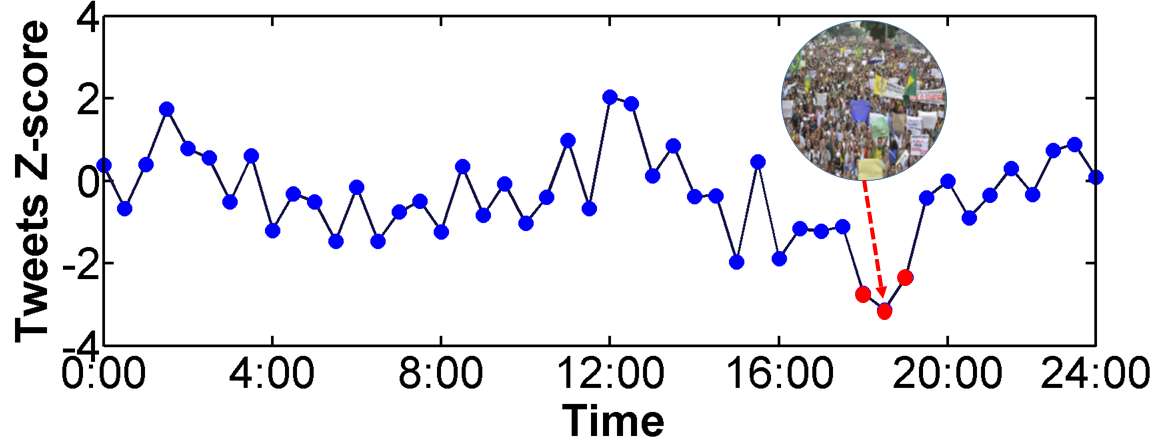
\includegraphics[width=4.5in]{figures/Natal_example1.png}
\caption{Detected group absenteeism in Natal, Brazil beginning at 6:00 PM on June 17, 2013. This absenteeism event coincides with a large protest that happened in the region.}
\label{fig:natal-protest}
\end{figure}


Developing a better appreciation of this phenomenon of unusually calm behavior online holds enormous potential for understanding localized, disruptive, societal events. In this chapter we focus on
absenteeism as a key phenomenon of interest and develop novel
group anomaly detection algorithms for this purpose.
An absenteeism event in a social network can be defined as an event which is characterized by a significant lull in activity such as a sudden, sharp decrease of Twitter volume within a short period of time (and which may precede a major burst in activity as people react to the event). This chapter presents the first study to systematically investigate group anomaly in location-based social networks (LBSNs). To appropriately incorporate absenteeism concepts into our detection approach, we must first address the following questions:

\begin{itemize}
\item How can we define/adapt anomaly detection algorithms to capture not just bursty situations
but also those that involve absenteeism?
\item At what scale should we model the absenteeism activity and how can we isolate the locus of
interest?
\item What is the most efficient way to select abnormal groups that are spatially and temporally localized?
\item How do we model an absenteeism signal for event detection? Even though we have clear examples of real world events that explain the observed absenteeism, not all absenteeism occurrences will be associated with underlying events and thus we must be able to differentiate between absenteeism and merely
noisy signals for successful event detection.
\end{itemize}

A graph wavelet approach offers several outstanding advantages to study the above questions, including scalability, localization, low computational complexity, and
compactness in defining groups. In this formalism, the data objects are embedded in a general graph as vertices. By employing wavelet transforms on the graph, we can construct a wavelet function with a graph structure. We propose the use of a graph anomaly index that depends on the graph structure in conjunction with an absenteeism score vector in order to define whether a graph is abnormal. When a graph is deemed to be exhibiting abnormal behavior, we can calculate its wavelet coefficient to identify the central node and its coverage area. This approach will enable us to select abnormal groups at different scales. Such group anomaly detection methods are varied and proven to be effective in detecting events such as protest marches and natural disasters.

%As for another abnormal scenarios such as natural disaster, we propose a two-pass group anomaly detection method that first detects absenteeism, and then checks if there is a subsequent burst in activity within a specific time period. By comparing correlations between the wavelet coefficients of both of these groups, we are able to capture a possible real world event.

Our contributions are thus:
\begin{itemize}
\item To the best of our knowledge this is the first study to utilize group absenteeism as a basis for event detection. By studying different types of group anomalies, either bursts or absenteeism, we demonstrate that these anomalies are indicative of key
events such as civil protests or natural disasters.
\item We incorporate graph wavelets as a mechanism to detect the most anomalous subgraphs at different scales. We demonstrate the power of this approach for social media analytics.
\item We define a graph anomaly index that can be used to determine whether a graph is abnormal. We then apply the graph wavelet to locate the central node and identify the abnormal groups.
%\item We propose a novel two-pass event detection method that uses correlation scores between the group depicting \textit{absenteeism} and the group demonstrating increased activity to probabilistically determine the likelihood of an event.
\end{itemize}

The rest of this chapter is organized as follows. Section~\ref{sec:related} reviews related work and existing methodologies and Section~\ref{sec:problem} formalizes the research problem. In Section~\ref{sec:algorithm}, we discuss the graph wavelet formalism for group anomaly detection.
%and subsequently demonstrate how it can be used for two-pass event detection.
Section~\ref{sec:experiment} extensive experiments testing our new approach's effectiveness for real-world event detection, and concludes with a summary of the research in Section~\ref{sec:conclusion}.



